
%%%%%%%%%%%%%%%%%%%%%%%%%%%%%%%%%%   ARBEITSLEBEN B3 - M4    %%%%%%%%%%%%%%%%%%%%%%%%%%%%%%%%%%%%%%%%%%%%%
\textsc{Aufgabe 1} 1) Gruppe: Vollzeitbeschäftigung und Normalarbeitsverhältnis S. 1-2 \quad 
\begin{myitemize}
    \item Die Hälfte der Vollzeitbeschäftigten möchte kürzer arbeiten.
    \item Ein Viertel derTeilzeitbeschäftigte möchte länger arbeiten.
    \item Über ein Drittel denkt wegen Arbeitszeitwünschen über eine Jobwechsel nach.
    \item 
\end{myitemize}

\textsc{Aufgabe 1} 2) Gruppe: Wunsch nach Arbeitszeitverkürzung M4 S. 2-4 \quad ---

\textsc{Aufgabe 1} 3) Gruppe: Arbeitszeit- und Arbeitsverdichtung M4 S. 4-5 \quad ---


\textsc{Aufgabe 3} 1) \quad ---

\textsc{Aufgabe 3} 2) \quad ---

\textsc{Aufgabe 3} 3) \quad ---
%%%%%%%%%%%%%%%%%%%%%%%%%%%%%%%%%%%%%%%%%%%%%%%%%%%%%%%%%%




%%%%%%%%%%%%% IN LINE 241 %%%%%%%%%%%%%%%%%%%%%%%%%%%%%%%%%%%%%%%%%%%%%%%%%%%
%%%%%%%%%%%%%%%%%%%%%%%%%%%%%%%%% INSERT HERE FROM FEHLER.TEX HWICH SAYS LINE 241 %%%%%%%%%%%%%%%%%%%%%%%%%%%



%%%%%%%%% eine schreckliche approximation %%%%%%%%%
\begin{align}
f(x) &\approx -3{,}1 \cdot 10^{-7} \cdot x^3 + 9 \cdot 10^{-4} \cdot x^2 - 0{,}146 \cdot x + 94 \\
     &\text{für } 0 < x < 1200
\end{align}
%%%%%%%%%%%%%%%%%%%%%%%%%%%%%%%%%%%%%%%%%

f (x) = x Df = {0 < x < 100} (1)
f (x) = 0, 2x + 80 Df = {100 < x < 520} (2)
f (x) = 0, 3x + 28 Df = {520 < x < 1000} (3)
f (x) = 0, 1x + 228 Df = {1000 < x < 1200} (4)




\addsec{Dokumentation der Nutzung von KI-basierten Anwendungen und Werkzeugen}
Die folgende Tabelle wurde in Anlehnung an die Vorlage der Universität Bremen erstellt:
\\

\footnotesize{
    \url{https://www.uni-bremen.de/zpa/formulare} führt zu: 
    \\

    \url{https://view.officeapps.live.com/op/view.aspx?src=https%3A%2F%2Fwww.uni-bremen.de%2Ffileadmin%2Fuser_upload%2Fsites%2Fzpa%2Fpdf%2Fallgemein%2FDokumentation_Nutzung_KI_-_AI_Use_Documentation.docx&wdOrigin=BROWSELINK} 
    \\
    
    beide 29.06.2025
    }

\clearpage
\newpage

\newgeometry{left=10mm, right=10mm, top=10mm, bottom=20mm} %%%

        \begin{landscape}
    \begin{table}
\centering 
\begin{tabularx}{\linewidth}{| >{\raggedright\arraybackslash} c || >{\raggedright\arraybackslash} X | >{\raggedright\arraybackslash} X | >{\raggedright\arraybackslash} X | >{\raggedright\arraybackslash} X | >{\raggedright\arraybackslash} X |} % {c|c|c|c|c|c} this was for tabular not tabularx

    \hline
                                & 
    KI-basiertes Hilfsmittel 
        
    AI-based Tool               & 
    Einsatzform 

    Purpose                     & 
    Betroffene Teile der Arbeit 
        
    Aspect of the Work Affected & 
    Beschreibung der Eingabe (Prompt) 
  
    Prompt (Entry)              & 
    Bemerkung 
    
    Comment                     \\ 
    \hline
    \hline
    %%%%%%%

    
    1                                                                                                                                           & 
    GitHub Copilot (Chat) in Visual Studio Code

    Inline Chat \& Chat on Secondary Sidebar

    mostly with GPT-4.1 as \gls{llm}                                                                                                            & 
    Fragen zu \LaTeX{} Code, keine inhaltlichen Fragen                                                                                          &
    alle, insbesondere \gls{zb} der Code zur Form dieser Tabelle oder Fragen zum Darstellen von eingebunden PDF-Seiten im Inhaltsverzeichnis    & 
    \gls{zb} \enquote{ia there \textbackslash{}vfill in latex?},  
    
    \enquote{what does \textbackslash{}arraybackslash in tabularx do?}, 
    
    \enquote{what can the parameter in lines 14 or 27 change?} oder
    
    \enquote{how do I make several entries to the toc like I treid in lines 26 to 62?}                                                          & 
    Es werden nicht alle Prompts aufgeführt. Es wurde ausschließlich für den Code Hintergrund benutzt und nie für den Inhalt. 
    
    Das Meiste wurde dann ohnehin doch wieder über Suchmaschinen und dann Foren und Anleitungen lesen erledigt. Häufig eben erst im Anschluss an das initiale Ausprobieren von \gls{ki} \\ 
    \hline
    %%%%%%%


    2                                                                                                                               &
    Visual Studio Code Autovervollständigung                                                                                        &
    Codevervollständigung und Autovervollständigung von einzelnen Worten, ähnlich dem Tippen auf Smartphones                        &
    alle                                                                                                                            &
    keine Prompts. 
    
    Bei der Eingabe \enquote{Effiz} wird dann \gls{zb} \enquote{Effizienz} vorgeschlagen und nach Druck auf Enter ausgeschrieben    &
    Die Grenze von maschinellem Lernen und Skripts oder überhaupt Software Hilfsmitteln ist fließend. Auch wenn schon länger existierende Autovervollständigungen für einzelne Worte keinen \gls{ki}-Boom und derartige gesellschaftliche Diskurse ausgelöst hat, wie es die \gls{llm} derzeit hervorrufen.                                             \\ 
    \hline

\pagebreak

    3                                               &
    ChatGPT.com                                     &
    Erstellen einer Graphik                         &
    Abbildung                                       &
    \enquote{Bitte plotte  die vier Funktionen unten in einer Abbildung. Beschrifte die x-Achse in hunderter Schritten. Mach keine Überschrift. Nenne die x-Achse anzurechnendes Einkommen in €. Nenne die y-Achse Absetzungsbetrag in €
    f (x) = x Df = {0 < x < 100} (1)
    f (x) = 0, 2x + 80 Df = {100 < x < 520} (2)
    f (x) = 0, 3x + 28 Df = {520 < x < 1000} (3)
    f (x) = 0, 1x + 228 Df = {1000 < x < 1200} (4)} &
    ---                                             \\
    \hline
    %%%%%%%

\end{tabularx}

\caption{Dokumentation der Nutzung von KI-basierten Anwendungen und Werkzeugen -- Documentation of the Use of AI-based Applications and Tools}

\label{KIHilfsmittel}

    \end{table}
        \end{landscape}

\restoregeometry %%%


% \footnote{\url{https://www.uni-bremen.de/zpa/formulare} führt zu \url{https://view.officeapps.live.com/op/view.aspx?src=https%3A%2F%2Fwww.uni-bremen.de%2Ffileadmin%2Fuser_upload%2Fsites%2Fzpa%2Fpdf%2Fallgemein%2FDokumentation_Nutzung_KI_-_AI_Use_Documentation.docx&wdOrigin=BROWSELINK} beide 29.06.2025}














\textsc{Aufgabe 2} a) \quad
ZU M1 VON DEMOKRATIE B3 - WAS GAR NICHT VERWENDET WIRD
\begin{myitemize}
    \item Mitbestimmung im Betrieb lässt Selbstwirksamkeit erfahren.
    \item Das kann sich auf die \enquote{parlametarische Demokratie} auswirken (\emph{spill-over Effekt})
    \item Menschen mit mehr Geld und Ressourcen wählen eher als Menschen mit wenig.
    \item Menschen ohen deutsche Staatsbürgherschasft dürfen auch überhaupt nicht wählen und arbeiten zusaätzlich häufig in prekäreren Verhältnissen. 
    \item Das ist für die demokratische Legitimation bedenklich.
    \item Lösungsansätze: 
        \begin{myitemize}
            \item Betriebliche Mitbestimmung stärken
            \item Schnellere Einbürgerungen 
            \item Repräsentation in den Parlamaenten von Frauen und Menschen mit Migrationsgeschichte ausbauen.
        \end{myitemize} 
\end{myitemize}


%%%%%%%%%%%%%%%%%%%%%%%%%%%%%%% KOMPETENZBLA %%%%%%%%%%%%%%%%%%%%%%%%%%%%%%%%%%%%%%%%%%%%%%%%%%%%%%%%%%%%%%%%%%%%%%%%%%%%%%%%%%%%%%%%%%%%%%%%%%%%%%%%%%%%%%%%%%%%
\subsubsection{Jonge, ich verliere mich in dem Komeptenzgebumsel; hier noch bla für weiter Schwafeln}
VIELLEICHT MAL EINE BRÜCKE ZU DEM EMOTIONS-BUMS SCHLAGEN? PASST HIER PRIMA REIN



Ein Politikunterricht, der nicht die politische Handlungsfähigkeit als Ziel hat, bleibt daher hinter seinem Potential zurück.



Eine Berufsschule ist zwar nicht mehr derart der Schulpflicht unterworfen, wie eine allgemeinbildende, aber die grundsätzlichen Strukturen, um welche es hier geht, sollten vergleichbar sein.

 \textcite[467-469]{Nonnenmacher2010}

Autorengruppe Fachdidaktik:
Wolfgang Sander, Sibylle Reinhardt, Andreas Petrik, Dirk Lange, Peter Henkenborg, Reinhold Hedtke, Tilman Grammes, Anja Besand
\autocite[]{Sander.2016}
digggaaaaahhh wohin gehört der bums?\autocite[]{Sander.2016}

%%%%%%%%%%%%%%%%%%%
ZITAT
Wolfgang Hilligen hatte in der schon erwähnten Untersuchung von 1955 Zur Auflösung der Fußnote[7] seine didaktischen Grundsätze bereits skizziert und damit zur Formulierung der Hessischen Richtlinien von 1957 beigetragen; seit diesem Jahr gibt es von ihm eines der bekanntesten Schulbücher („Sehen-Beurteilen-Handeln“) für den politischen Unterricht. Seine didaktische Konzeption entstand nicht aus einer vorgängigen wissenschaftlich-systematischen Überlegung, sondern umgekehrt aus den Schwierigkeiten der Unterrichtspraxis selbst, für deren Lösung er nach einer verallgemeinerungsfähigen, d. h. auch für andere Lehrer in gleicher Lage nützlichen Theorie suchte. Weil er diese im Laufe der Zeit immer wieder modifizierte und präzisierte, ist sein Wirken bis in die achtziger Jahre hinein eine wichtige Quelle für das Studium der Schwierigkeiten, die angesichts fortschreitender politischer und wissenschaftlicher Veränderungen mit einem solchen Vorhaben verbunden sind.  (Giesecke 1999, S. 15)

\enquote{Sehen-Beurteilen-Handeln} auch schon in den 50er Jahren ein Ding, guck hier \autocite[15]{Giesecke.1999}

ZITAT
3. Politisches und pädagogisches Handeln unter liegen unterschiedlichen Strategien und Erfolgskriterien. Das eine ist darauf aus, die Wirklichkeit zu verändern, das andere, sie im Rahmen geplanter Lehr- und Lernarrangements verständlich zu machen. Welche Schlußfolgerungen die Lernen den daraus ziehen, müssen sie selbst entscheiden. Insofern bleibt immer fraglich, ob Lehrziele auch tatsächlich zu Lernzielen werden. Die Didaktik kann von sich aus die Wirklichkeit nicht gestalten, über die sie aufklären will. \autocite[22]{Giesecke.1999}


Fischer Prinzip \autocite[]{Grammes.2005}

ZITAT
 Zum Verhandeln gehören neben argumentativen Strategien, die der konsensuellen Entscheidungsfindung dienen, auch Strategien, die durch den Einsatz von Machtpotenzialen, Konfliktfähigkeit, ökonomischen Ressourcen oder Tausch versuchen, Verhandlungsprozesse abzukürzen und zu hierarchisch autoritären oder hierarchisch majoritären Entscheidungen zu gelangen. Diese lassen sich im Unterricht zwar nicht erfahren, sollten aber gewusst werden. Entscheiden als Teil des realen partizipativen politischen Handelns lässt sich im Unterricht nur begrenzt fördern. Auch wenn Entscheiden durch kooperative oder handlungsorientierte Methoden geübt werden kann, bleibt es gegenüber der realen Politik unterkomplex. Allerdings lassen sich an konkreten politischen Fällen, Problemen, Konflikten oder Entscheidungsprozessen unterschiedliche Strategien und ihre Wirksamkeit analysieren, deren Ergebnisse den Lernenden dann als Fachwissen zur Verfügung stehen. (Massing 2012, S. 27)

JOOONGE, DAS IST AUCH BEI KAPITEL RELFEXION

bin bei gloe2020 s. 116 pdf118

% \subsubsection{Brudi, SOLL DAS VIELLEICHT NOCH IN DAS ELLENLANGE KOMPETENZKAPITEL? KA MAN}
% Massing meint Verhandeln mit Macht kann nicht erfahren werden. Was ist mit DSP diggi. \autocite[27]{Massing2012}
% Gefunden nach \autocite[111]{Gloe2020}
% \enquote{Die Strategien des Verhandelns, neben Argumentationsstrategien z. B. auch der Einsatz von Machtpotenzialen u. Ä., können in Lernprozessen »nicht erfahren, sollten aber gewusst werden« (Massing 2012: 27). Ebenso lässt sich die Kompetenzfacette Entscheiden nur begrenzt in Lernprozessen fördern: »Auch wenn Entscheiden durch kooperative oder handlungsorientierte Methoden geübt werden kann, bleibt es gegenüber der realen Politik unterkomplex« (ebd.).}

ZITAT
Das Leitmotiv einer Pädagogik der Lernhilfe hat sicher den Vorteil einer pragmatischen Sicht auf den Lehrerberuf. Problematisch an dem Modell ist allerdings, dass es die Schule von den sozialen Problemen von Schülerinnen und Schülern in der heutigen Gesellschaft entkoppelt (Böhnisch/Schroer 2011). \autocite[51]{Sander.2016}

Kompetenzen können kritisiert werden, es gibt Ähnlichkeiten. \enquote{Sie leisten die Verbindung zwischen den jeweiligen Bildungszielen der Fächer und den Aufgabenstellungen des Unterrichts (Detjen et al. 2012, S. 20)} \autocite[18]{Massing.2022}

Ähnlich vernichtend wie \textcite[][]{Roler2016} den Beutelsbacher Konsens auseinanderbastelt, ließe sich der nur bemüht als praxisnah zu empfindenden Debatte um Kompetenzen gegenüberstehen. Allerdings 
%%%%%%%%%%%%%%%%%%%%%%%%%%%%%%%%%%%%%%%%%%%%%%%%%%%%%%%%%%%%%%%%%%%%%%%%%%%%%%%%%%%%%%%%%%%%%%%%%%%%%%%%%%%%%%%%%%%%%%%%%%%%%%%%%%%%%%%%%%%%%%%%%%%%%%%%%%%%%%%%%%%%%%%%%%%%%%%%%%%%%%%%%%%%%%%%%%%%%%%%%%%%%%%%%%%%%%%%%%%%%%%%%%%%%%%%%%%%%%%%%%%%%%%%%%%%%%%%%%%%%%%%%%%%%%%%%%%%%%%%%%







%%%%%%%%%%%%%%%%%%%%%%%%% TABELLENZEILE FÜR  ERWARTUNGSHORIZONT %%%%%%%%%%%%%%%%%%%%%%%%%%%%%%%%%%
     2 & 
    Copilot in Microsoft Edge & 
    Zusammenfassung von Texten & 
    Die Erwartungshorizonte.       
    \gls{ki}-Einsatz ist an den jeweiligen Stellen der Arbeit direkt angegeben &
    \enquote{fasse mir stichpunktartig die punkte des pdf zusammen} & 
    \\
    \hline




%%%%%%%%%% DIESE Version MACHT FEHLER wegen der Fußnoten %%%%%%%%%%%%%%%%%%%%%%%%%
Beim \gls{bmas} findet sich tatsächlich eine nette Übersicht vom \enquote{Referenzentwurf} über den \enquote{Kabinettsbeschluss} bis zum \enquote{Abschluss des Gesetzes}\footnote{
    \url{https://www.bmas.de/DE/Service/Gesetze-und-Gesetzesvorhaben/arbeitsschutzkontrollgesetz.html} 19.06.2025
}. 
Alle Schriftstücke sind, wie es sein sollte, verlinkt. Der Referenzentwurf vom \gls{bmas}\footnote{
    \url{https://www.bmas.de/SharedDocs/Downloads/DE/Gesetze/Regierungsentwuerfe/reg-arbeitsschutzkontrollgesetz.pdf?__blob=publicationFile&v=3} 19.06.2025
} ist dabei einfach brav als PDF anzutreffen \autocite{BMAS-21.07.2020}. 
Die Drucksache\footnote{
    \url{https://dserver.bundestag.de/btd/19/219/1921978.pdf} 19.06.2025
} des Bundestages hingegen ist kopiergeschützt, wtf \autocite{Bundestag.31.08.2020}?
Das Bundesgesetzblatt ist zwar ein eher maschinenlesbarer Link\footnote{
    \url{https://www.bgbl.de/xaver/bgbl/start.xav?start=%2F%2F%2A%5B%40attr_id%3D%27bgbl120s3334.pdf%27%5D#/switch/tocPane?_ts=1750343088377} 19.06.2025
} aber hat immerhin einen netten Viewer mit ziemlich guter Suchfunktion integriert und ist damit nicht kopiergeschützt \autocite{BGBl.2020-I-Nr67}. 
%%%%%%%%%%%%%%%%%%%%%%%%%%%%%%%%%%%%%%%%%%%%%%%%%%%%%%%%%%%%%%%%%%%%%%%%%%%%%%%%%%%%%%%%%%%%%%%%%%%%%%%%%%%%%%


%%%%%%%%%%%%%%%% ZWEITE VERSION OHNE FUßNOTEN, die geht %%%%%%%%%%%%%%%%%%%%%%%%%%%%%%%%%%%%%%%%%%%%%%%%%
Beim \gls{bmas} findet sich tatsächlich eine nette Übersicht vom \enquote{Referenzentwurf} über den \enquote{Kabinettsbeschluss} bis zum \enquote{Abschluss des Gesetzes}.
Alle Schriftstücke sind, wie es sein sollte, verlinkt. Der Referenzentwurf vom \gls{bmas} ist dabei einfach brav als PDF anzutreffen \autocite{BMAS-21.07.2020}. 
Die Drucksache des Bundestages hingegen ist kopiergeschützt, wtf \autocite{Bundestag.31.08.2020}?
Das Bundesgesetzblatt ist zwar ein eher maschinenlesbarer Link, aber hat immerhin einen netten Viewer mit ziemlich guter Suchfunktion integriert und ist damit nicht kopiergeschützt \autocite{BGBl.2020-I-Nr67}. 
%%%%%%%%%%%%%%%%%%%%%%%%%%%%%%%%%%%%%%%%%%%%%%%%%%%%%%%%%%%%%%%%%%%%%%%%%%%%%%%%%%%%%%%%%%%%%%%%%%%%%%%%%


%%%%%%%%%%%%%%%%%%%%%%%%%%%%%%%%%%%%
\newenvironment{myenumerate}
{ \begin{enumerate}
    \setlength{\itemsep}{0pt}
    \setlength{\parskip}{0pt}
    \setlength{\parsep}{0pt}     }
{ \end{enumerate}                } 
%%%%%%%%%%%%%%%%%%%%%%%%%%%%%%%%%%%


%%%%%%%%%%%%% FUNKTIONIERENDE VERSION %%%%%%%%%%%%%%%%%%%%%%%%%%%%%%%%%%%%%%%%%%%%%%%%%%%%%%%%%%%%%%%%%%%%%%%%%%%%
        \begin{landscape}
    \begin{table}
\centering 
\begin{tabularx}{\linewidth}{| X | X | X | X | X | X |} % {c|c|c|c|c|c} this was for tabulat without x

    \hline
     & 
    KI-basiertes Hilfsmittel 
        
    AI-based Tool & 
    Einsatzform 

    Purpose & 
    Betroffene Teile der Arbeit 
        
    Aspect of the Work Affected & 
    Beschreibung der Eingabe (Prompt) 
  
    Prompt (Entry) & 
    Bemerkung 
    
    Comment\\
    \hline
    \hline
    
    1 & 
    Copilot in Visual Studio Code
    
    mostly with GPT-4.1 as \gls{llm} & 
    Fragen zu \LaTeX Code, keine inhaltlichen Fragen &
    alle, insbesondere \gls{zb} der Code zur Form dieser Tabelle & 
    \gls{zb} \enquote{ia there \textbackslash{}vfill in latex?} & 
    Es werden nicht alle Prompts aufgeführt. Es wurde ausschließlich für den Code Hintergrund benutzt und nie für den Inhalt. 
    
    Das Meiste wurde dann ohnehin doch wieder über Suchmaschinen und Anleitungen lesen erledigt. Häufig eben im Anschluss an das Ausprobieren von \gls{ki} \\
    \hline


     2 & 
    Copilot in Microsoft Edge & 
    Zusammenfassung von Texten & 
    Die Erwartungshorizonte       
    An den jeweiligen Stellen der Arbeit direkt angegeben &
    \enquote{fasse mir stichpunktartig die punkte des pdf zusammen} & 
    \\

\end{tabularx}

\caption{Dokumentation der Nutzung von KI-basierten Anwendungen und Werkzeugen -- Documentation of the Use of AI-based Applications and Tools}

\label{KIHilfsmittel}

    \end{table}

        \end{landscape}
%%%%%%%%%%%%%%%%%%%%%%%%%%%%%%%%%%%%%%%%%%%%%%%%%%%%%%%%%%%%%%%%%%%%%%%%%%%%%%%%%%%%%%%%%%%%%%%%%%%%%%%%%%%%%%%%%%%%%%%%%%%%%%%%%%%%%%%



%%%%%%%%%% ALTE VERSION %%%%%%%%%%%%%%%%%%%%%%%%%%%%%%%%%%%%%%%%%%%%%%%%%%%%%%%%%%%%%%%%%%%%%%%%%%%%%%%
\begin{landscape}

\begin{table}
    \centering
    \begin{tabularx{\linewidth}{ 
        | >{\raggedright\arraybackslash}X 
        | >{\raggedright\arraybackslash}X 
        | >{\raggedright\arraybackslash}X 
        | >{\raggedright\arraybackslash}X 
        | >{\raggedright\arraybackslash}X 
        | >{\raggedright\arraybackslash}X | 
        }
        } % {c|c|c|c|c|c} this was for tabulat without x
        
        & 
         KI-basiertes Hilfsmittel AI-based Tool & 
         Einsatzform Purpose & 
         Betroffene Teile der Arbeit Aspect of the Work Affected & 
         Beschreibung der Eingabe (Prompt) Prompt (Entry) & 
         Bemerkung Comment\\
        \hline
        
        1 & 
        Copilot in Visual Studio Code
        
        mostly with GPT-4.1 as \gls{llm} & 
        alle &
        Fragen zu LaTeX Code, keine inhaltlichen Fragen & 
        \gls{zb} \enquote{ia there \textbackslash{}vfill in latex?} & 
        es werden nicht alle Prompts aufgeführt. Es wurde ausschließlich für den Code Hintergrund benutzt und nie für den Inhalt. Das Meiste wurde dennoch über Suchmaschinen und Anleitungen lesen erledigt. Meist auch noch im Anschluss an das Ausprobieren von \gls{ki} \\


        2 & 
        Copilot in Microsoft Edge & 
        Zusammenfassung von Texten, meist bei den Erwartungshorizonten. An den jeweiligen Stellen der Arbeit direkt angegeben & 
        \enquote{fasse mir stichpunktartig die punkte des pdf zusammen} & 
         & \\
    \end{tabularx}
    \caption{Dokumentation der Nutzung von KI-basierten Anwendungen und Werkzeugen -- Documentation of the Use of AI-based Applications and Tools}
    \label{KIHilfsmittel}
\end{table}

\end{landscape}
%%%%%%%%%%%%%%%%%%%%%%%%%%%%%%%%%%%%%%%%%%%%%%%%%%%%%%%%%%%%%%%%%%%%%%%%%%%%%%%%%%%%%%%%%%%%%%%%%%%%%%%%%%%%%%%
Allgemeine Entwicklungen
\begin{myitemize}
\item Rückgang der Berufskrankheiten-Anzeigen in Bremen 2017 um 20\% gegenüber 2016 – Ursache unklar.
\item 2017: 899 Verdachtsanzeigen, 401 Anerkennungen, 139 neue Renten, 100 Todesfälle.
\item Bremen hat im Vergleich zum Bund ein ungünstigeres Verhältnis von Anzeigen zu Todesfällen.
\end{myitemize}


Hauptursachen für Berufskrankheiten
\begin{myitemize}
\item Asbestbedingte Erkrankungen dominieren (z. B. Asbestose, Mesotheliom).
\item Weitere häufige Erkrankungen: Hautkrankheiten, Lärmschwerhörigkeit, Hautkrebs durch UV-Strahlung.
\item Asbest: Ursache für 94 von 100 Todesfällen 2017.
\end{myitemize}


Geschlechtsspezifische Unterschiede
\begin{myitemize}
\item Frauen: häufig betroffen durch Haut-, Infektions- und Wirbelsäulenerkrankungen in frauendominierten Berufen.
\item Männer: häufiger betroffen durch asbestbedingte Erkrankungen, Lärm, UV-Strahlung – typisch für Industrie und Bau.
\end{myitemize}


Anerkennungsverfahren & Hürden
\begin{myitemize}
\item Berufskrankheit = juristischer Begriff, nicht medizinisch.
\item Hohe Beweislast bei Betroffenen: Nachweis der beruflichen Ursache erforderlich.
\item Verfahren oft langwierig, Anerkennung schwierig, besonders bei fehlender Dokumentation oder Betriebsauflösung.
\item Manche Krankheiten (z.B. chronisches Ekzem) nur anerkennbar nach Tätigkeitsaufgabe.
\end{myitemize}


Beratung & Unterstützung
\begin{myitemize}
\item Beratungsstelle der Arbeitnehmerkammer Bremen bietet kostenlose Hilfe.
\item 2018: 260 Beratungen, v.a. zu Asbest, Muskel-Skelett-Erkrankungen, Lärm, Krebs, Asthma.
\item Fehlende unabhängige arbeitsmedizinische Expertise seit Wegfall des Landesgewerbearztes.
\end{myitemize}


Arbeitsschutz & Prävention
\begin{myitemize}
\item Schwerpunktaktion 2018 zu UV-Strahlung: große Defizite bei Prävention in Betrieben.
\item Nur 41 von 115 Betrieben hatten Gefährdungsbeurteilung zu UV-Strahlung.
\item Schutzmaßnahmen oft unzureichend oder von Beschäftigten selbst finanziert.
\end{myitemize}


Politische Forderungen & Handlungsbedarf
\begin{myitemize}
\item Anerkennungssystem muss reformiert werden: z.B. Beweiserleichterung bei Beweisnot.
\item Erweiterung der Berufskrankheiten-Liste notwendig (z.B. frauentypische Erkrankungen).
\item Bessere Ausstattung der Gewerbeaufsicht und Rückkehr eines Landesgewerbearztes gefordert.
\item Systematischer Arbeitsschutz und gezielte Prävention müssen gestärkt werden.
\end{myitemize}
%%%%%%%%%%%%%%%%%%%%%%%%%%%%%%%%%%%%%%%%%%%%%%%%%%%%%%%%%%%%%%%%%%%%%%%%%%%%%%%%%%%%%%%%%%%%%%%%%%%%%%%%%%%%%%%%%%%%%%%%%%%%%%%%
Aufgabe 1 - Die Lösung zu Aufgabe 1 ist von Copilot zusammengefasst und neu formatiert:

\textbf{Allgemeine Entwicklungen}
\begin{myitemize}
\item Rückgang der Berufskrankheiten-Anzeigen in Bremen 2017 um 20\% gegenüber 2016 – Ursache unklar.
\item 2017: 899 Verdachtsanzeigen, 401 Anerkennungen, 139 neue Renten, 100 Todesfälle.
\item Bremen hat im Vergleich zum Bund ein ungünstigeres Verhältnis von Anzeigen zu Todesfällen.
\end{myitemize}


\textbf{Hauptursachen für Berufskrankheiten}
\begin{myitemize}
\item Asbestbedingte Erkrankungen dominieren (z.B. Asbestose, Mesotheliom).
\item Weitere häufige Erkrankungen: Hautkrankheiten, Lärmschwerhörigkeit, Hautkrebs durch UV-Strahlung.
\item Asbest: Ursache für 94 von 100 Todesfällen 2017.
\end{myitemize}


\textbf{Geschlechtsspezifische Unterschiede}
\begin{myitemize}
\item Frauen: häufig betroffen durch Haut-, Infektions- und Wirbelsäulenerkrankungen in frauendominierten Berufen.
\item Männer: häufiger betroffen durch asbestbedingte Erkrankungen, Lärm, UV-Strahlung – typisch für Industrie und Bau.
\end{myitemize}


\textbf{Anerkennungsverfahren \& Hürden}
\begin{myitemize}
\item Berufskrankheit = juristischer Begriff, nicht medizinisch.
\item Hohe Beweislast bei Betroffenen: Nachweis der beruflichen Ursache erforderlich.
\item Verfahren oft langwierig, Anerkennung schwierig, besonders bei fehlender Dokumentation oder Betriebsauflösung.
\item Manche Krankheiten (z.B. chronisches Ekzem) nur anerkennbar nach Tätigkeitsaufgabe.
\end{myitemize}


\textbf{Beratung \& Unterstützung}
\begin{myitemize}
\item Beratungsstelle der Arbeitnehmerkammer Bremen bietet kostenlose Hilfe.
\item 2018: 260 Beratungen, v.a. zu Asbest, Muskel-Skelett-Erkrankungen, Lärm, Krebs, Asthma.
\item Fehlende unabhängige arbeitsmedizinische Expertise seit Wegfall des Landesgewerbearztes.
\end{myitemize}


\textbf{Arbeitsschutz \& Prävention}
\begin{myitemize}
\item Schwerpunktaktion 2018 zu UV-Strahlung: große Defizite bei Prävention in Betrieben.
\item Nur 41 von 115 Betrieben hatten Gefährdungsbeurteilung zu UV-Strahlung.
\item Schutzmaßnahmen oft unzureichend oder von Beschäftigten selbst finanziert.
\end{myitemize}


\textbf{Politische Forderungen \& Handlungsbedarf}
\begin{myitemize}
\item Anerkennungssystem muss reformiert werden: z.B. Beweiserleichterung bei Beweisnot.
\item Erweiterung der Berufskrankheiten-Liste notwendig (z.B. frauentypische Erkrankungen).
\item Bessere Ausstattung der Gewerbeaufsicht und Rückkehr eines Landesgewerbearztes gefordert.
\item Systematischer Arbeitsschutz und gezielte Prävention müssen gestärkt werden.
\end{myitemize}
%%%%%%%%%%%%%%%%%%%%%%%%%%%%%%%%%%%%%%%%%%%%%%%%%%%%%%%%%%%%%%%%%%%%%%%


%%----------------------------------------------%%
\usepackage[]{minitoc}
\setcounter{secttocdepth}{4}
\setlength{\stcindent}{24pt}

\dosecttoc
\dosectlof
\dosectlot

%%----------------------------------------------%%
\secttoc
%%----------------------------------------------%%



%%%%%%%%%%%%%%%%%%%    BBK    %%%%%%%%%%%%%%%%%%%%%%%%%
\begin{quote}
    \textbf{1. Überwältigungsverbot.}

    Es ist nicht erlaubt, den Schüler - mit welchen Mitteln auch immer - im Sinne erwünschter Meinungen zu überrumpeln und damit an der \enquote{Gewinnung eines selbständigen Urteils} zu hindern. Hier genau verläuft nämlich die Grenze zwischen Politischer Bildung und Indoktrination. Indoktrination aber ist unvereinbar mit der Rolle des Lehrers in einer demokratischen Gesellschaft und der - rundum akzeptierten - Zielvorstellung von der Mündigkeit des Schülers. 

    \textbf{2. Was in Wissenschaft und Politik kontrovers ist, muss auch im Unterricht kontrovers erscheinen.}

    Diese Forderung ist mit der vorgenannten aufs engste verknüpft, denn wenn unterschiedliche Standpunkte unter den Tisch fallen, Optionen unterschlagen werden, Alternativen unerörtert bleiben, ist der Weg zur Indoktrination beschritten. Zu fragen ist, ob der Lehrer nicht sogar eine Korrekturfunktion haben sollte, d.h. ob er nicht solche Standpunkte und Alternativen besonders herausarbeiten muss, die den Schülern (und anderen Teilnehmern politischer Bildungsveranstaltungen) von ihrer jeweiligen politischen und sozialen Herkunft her fremd sind. Bei der Konstatierung dieses zweiten Grundprinzips wird deutlich, warum der persönliche Standpunkt des Lehrers, seine wissenschaftstheoretische Herkunft und seine politische Meinung verhältnismäßig uninteressant werden. Um ein bereits genanntes Beispiel erneut aufzugreifen: Sein Demokratieverständnis stellt kein Problem dar, denn auch dem entgegenstehende andere Ansichten kommen ja zum Zuge. 
    
    \textbf{3. Der Schüler muss in die Lage versetzt werden, eine politische Situation und seine eigene Interessenlage zu analysieren,} 

    sowie nach Mitteln und Wegen zu suchen, die vorgefundene politische Lage im Sinne seiner Interessen zu beeinflussen. Eine solche Zielsetzung schließt in sehr starkem Maße die Betonung operationaler Fähigkeiten ein, was eine logische Konsequenz aus den beiden vorgenannten Prinzipien ist. Der in diesem Zusammenhang gelegentlich - etwa gegen Herman Giesecke und Rolf Schmiederer - erhobene Vorwurf einer \enquote{Rückkehr zur Formalität}, um die eigenen Inhalte nicht korrigieren zu müssen, trifft insofern nicht, als es hier nicht um die Suche nach einem Maximal-, sondern nach einem Minimalkonsens geht. 
    
    \autocite[Im Original mit anderen Hervorhebungen:][179-180]{Wehling1977}
\end{quote}
%%%%%%%%%%%%%%%%%%%%%












%%%%%%%%%%%%%%%%%%%%%%%%%%%%%%%%%%%%%%     WIRTSCHAFTSPOLITIK IM APENDIX ALS PDF       %%%%%%%%%%%%%%%%%
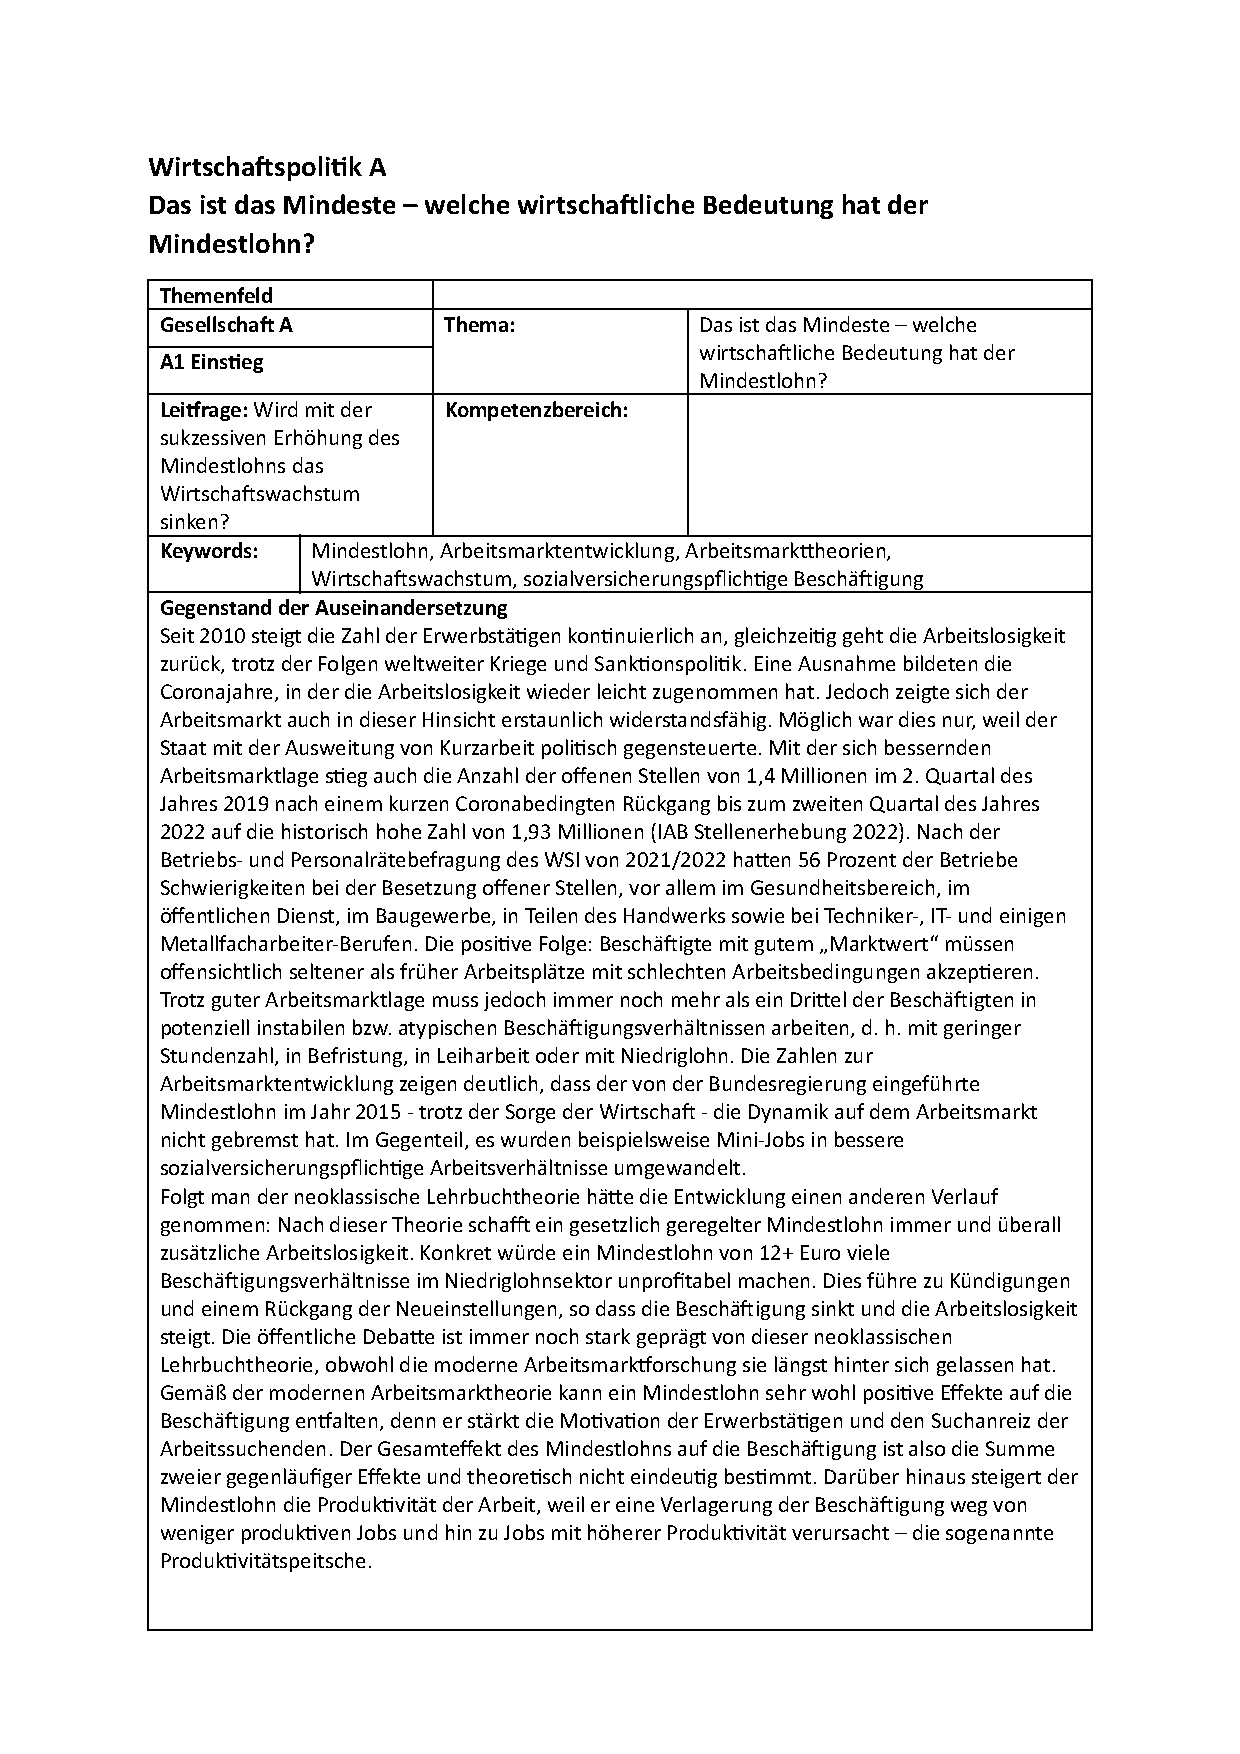
\includepdf[
    nup=2x1, 
    addtotoc={
    1, subsection, 2, Wirtschaftspolitik A1, WIRTSCHAFTSPOLITIK-A1, 
    3, subsection, 2, Wirtschaftspolitik A2, WIRTSCHAFTSPOLITIK-A2, 
    5, subsection, 2, Wirtschaftspolitik A3, WIRTSCHAFTSPOLITIK-A3, 
    7, subsection, 2, Wirtschaftspolitik B1, WIRTSCHAFTSPOLITIK-B1, 
    9, subsection, 2, Wirtschaftspolitik B2, WIRTSCHAFTSPOLITIK-B2, 
    11, subsection, 2, Wirtschaftspolitik C1, WIRTSCHAFTSPOLITIK-C1, 
    13, subsection, 2, Wirtschaftspolitik C2, WIRTSCHAFTSPOLITIK-C2
    }
]
{WIRTSCHAFTSPOLITIK.pdf} 
%%%%%%%%%%%%%%%%%%%%%%%%